% SECTION: Probabilistische PCA (PPCA)
\section{Probabilistische PCA (PPCA)}

\divider

% SUBSECTION: PPCA Modell
\subsection{PPCA Modell}

% PCA als latent Variable Model
\begin{frame}{PCA als latent Variable Model}{}
	\begin{itemize}
		\item Wir modellieren die Repräsentation der Daten im Principal Subspace als latente Variablen $\bz \in \R^D$.
		\item Für die Verteilung von $\bz$ gelte
		\begin{equation} \label{eq:ppca-dist-z}
			\bz \sim \norm(\0, \bI).
		\end{equation}
		\item Zudem führen wir die bedingte Verteilung von $\bx \in \R^M$ gegeben $\bz$ wie folgt ein
		\begin{equation} \label{eq:ppca-dist-x-given-z}
			\bx \mid \bz \sim \norm\bigl( \bW \bz + \bmu, \sigma^2 \bI \bigr).
		\end{equation}
		\item Die Spalten der Matrix $\bW \in \R^{M \times D}$ spannen hierbei den Principal Subspace auf.
		\item Es ist $\bmu \in \R^M$.
		\item Der Parameter $\sigma^2$ beeinflusst die Varianz der bedingten Verteilung \eqref{eq:ppca-dist-x-given-z}.
	\end{itemize}
\end{frame}


% PPCA als generatives Modell
\begin{frame}{PPCA als generatives Modell}{}
	Die PPCA kann als \keyword{generatives Modell} aufgefasst werden:
	\begin{itemize}
		\item Zunächst wählen wir ein $\bz$ gemäß \eqref{eq:ppca-dist-z}.
		\item Dann ziehen wir die beobachtete Variable $\bx$ aus der Verteilung \eqref{eq:ppca-dist-x-given-z}.
		\item Hierbei ergibt sich der Wert für $\bx$ gemäß
		\begin{equation} \label{eq:ppca-comp-x}
			\bx = \bW \bz + \bmu + \beps.
		\end{equation}
		\item $\beps \sim \norm\bigl( \0, \sigma^2 \bI \bigr)$ ist hierbei \textit{additives normalverteiltes Datenrauschen},
			welches durch den Parameter $\sigma^2$ in \eqref{eq:ppca-dist-x-given-z} beeinflusst wird.
	\end{itemize}
	
	\begin{boxGray}
		Das Mapping der Daten in den Principal Subspace erhalten wir mit dem Satz von Bayes.
	\end{boxGray}
\end{frame}


% PPCA als generatives Modell (Forts.)
\begin{frame}{PPCA als generatives Modell}{}
	\begin{figure}
		\centering
		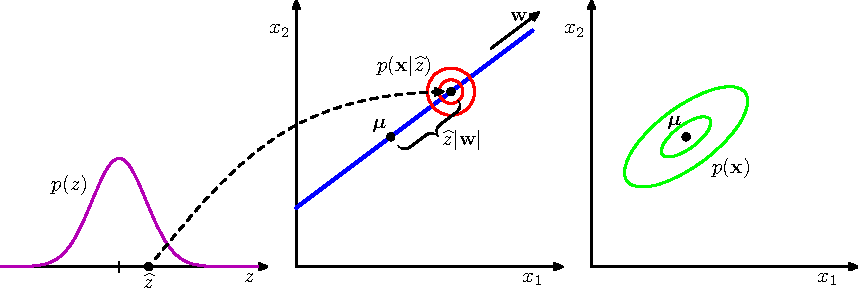
\includegraphics[scale=0.9]{./img/ppca/ppca_generative}
		\caption{PPCA als generatives Modell. Siehe \cite{Bishop2006}, Seite 572.}
	\end{figure}
\end{frame}


% SUBSECTION: Bestimmung der Verbunddichte
\subsection{Bestimmung der Verbunddichte}

% Bestimmung der Verbunddichte
\begin{frame}{Bestimmung der Verbunddichte}{}
	\begin{itemize}
		\item Für die weiteren Ausführungen benötigen wir die Verbunddichte $p(\bz, \bx)$
			der beobachteten und latenten Variablen.
		\item Mit der Produktregel für Wahrscheinlichkeiten ist
		\begin{equation} \label{eq:ppca-joint-dist}
			p(\bz, \bx) = \normdense(\bx \mid \bz) \cdot \normdense(\bz).
		\end{equation}
		\item Da es sich bei \eqref{eq:ppca-joint-dist} um ein Produkt von Normalverteilungen handelt,
			sind die Zufallsvariablen auch gemeinsam normalverteilt.
		\item Es ist also $p(\bz, \bx) = \normdense(\bz, \bx; \bnu, \bSigma)$ beziehungsweise
		\begin{equation}
			\begin{pmatrix} \bz \\ \bx \end{pmatrix} \sim \norm(\bnu, \bSigma).
		\end{equation}
	\end{itemize}
\end{frame}


% Bestimmung der Verbunddichte (Forts.)
\begin{frame}{Bestimmung der Verbunddichte (Forts.)}{}
	Wir bestimmen zunächst den Parameter $\bnu = (\bmu_{\bz}, \bmu_{\bx})^\top$:
	\begin{itemize}
		\item Mit der Linearität des Erwartungswerts und den obigen Definitionen --
			insbesondere die Definitionen \eqref{eq:ppca-dist-z} und \eqref{eq:ppca-comp-x} -- gilt
		\begin{align*}
			\E[\bz]
				&= \0
		\\[2mm]
			\E[\bx]
				&= \E[\bW \bz + \bmu + \beps]
				= \bW \underbracket{\E[\bz]}_{= \0} + \E[\bmu] + \underbracket{\E[\beps]}_{= \0}
				= \bmu.
		\end{align*}
		\item Zusammenfassend gilt also
		\begin{equation} \label{eq:ppca-expectation-joint-dist}
			\bnu
				= \E\left[ \begin{pmatrix} \bz \\ \bx \end{pmatrix} \right]
				= \begin{pmatrix} \E[\bz] \\ \E[\bx] \end{pmatrix}
				= \begin{pmatrix} \0 \\ \bmu \end{pmatrix}.
		\end{equation}
	\end{itemize}
\end{frame}


% Bestimmung der Verbunddichte (Forts.)
\begin{frame}{Bestimmung der Verbunddichte (Forts.)}{}
	Nun bestimmen wir den Parameter
		$\bSigma = \begin{pmatrix} \bSigma_{\bz\bz} & \bSigma_{\bz\bx} \\ \bSigma_{\bx\bz} & \bSigma_{\bx\bx} \end{pmatrix}$:
	\begin{itemize}
		\item Zunächst ist $\bSigma_{\bz\bz} = \E\bigl[ (\bz - \E[\bz]) (\bz - \E[\bz])^\top \bigr] = \E[\bz \bz^\top] = \D[\bz] = \bI$.
		\item Ferner ist
		\begin{align*}
			\bSigma_{\bz \bx}
				&= \E\bigl[ (\bz - \E[\bz]) (\bx - \E[\bx])^\top \bigr]
		\\[2mm]
				&= \E\bigl[\bz (\bW \bz + \bmu + \beps - \E[\bW \bz + \bmu + \beps])^\top \bigr]
		\\[2mm]
				&= \E\bigl[\bz (\bW \bz + \beps)^\top \bigr]
					= \E\bigl[ \bz \bz^\top \bW^\top + \bz \beps^\top \bigr]
					= \E\bigl[ \bz \bz^\top \bigr] \bW^\top  + \E\bigl[ \bz \bigr] \cdot \E\bigl[ \beps^\top \bigr]
		\\[2mm]
				&= \bW^\top.
		\end{align*}
		\item Aus Symmetriegründen gilt $\bSigma_{\bx \bz} = \bW$.
	\end{itemize}
\end{frame}


% Bestimmung der Verbunddichte (Forts.)
\begin{frame}{Bestimmung der Verbunddichte (Forts.)}{}
	\begin{mytask}
		Zeigen Sie durch analoge Rechnung, dass $\bSigma_{\bx\bx} = \bW \bW^\top + \sigma^2 \bI$ gilt.
	\end{mytask}
	
	\begin{boxGray}
		\textbf{Zusammenfassung:} Für die gemeinsame Verteilung von $\bz$ und $\bx$ erhalten wir also
		\begin{equation} \label{eq:ppca-joint-dist}
			\begin{aligned}
				\begin{pmatrix} \bz \\ \bx \end{pmatrix}
					&\sim \norm(\bnu, \bSigma)
			\\[2mm]
				\bnu
					&\coloneqq \begin{pmatrix} \0 \\ \bmu \end{pmatrix}
			\\[2mm]
				\bSigma
					&\coloneqq \begin{pmatrix} \bI & \bW^\top \\ \bW & \bW \bW^\top + \sigma^2 \bI \end{pmatrix}.
			\end{aligned}
		\end{equation}
	\end{boxGray}
\end{frame}


% SUBSECTION: Bestimmung des Posteriors der latenten Variablen
\subsection{Bestimmung des Posteriors der latenten Variablen}

% Woodbury Matrix-Identität
\begin{frame}{Woodbury Matrix-Identität}{}
	\begin{mytheo}[th:ppca-woodbury]
		Es gilt die \keyword{Woodbury Matrix-Identität}
		\begin{equation*}
			\bigl( \bA + \bB \bD^{-1} \bE \bigr)^{-1}
				= \bA^{-1} - \bA^{-1} \bB \bigl( \bD + \bE \bA^{-1} \bB \bigr)^{-1} \bE \bA^{-1},
		\end{equation*}
		wobei $\bA, \bB, \bD$ und $\bE$ Matrizen geeigneter Form sind.
	\end{mytheo}
	
	\begin{myproof}
		Der Beweis erfolgt durch Nachrechnen, indem man beide Seiten der Gleichung mit $\bA + \bB \bD^{-1} \bE$
		multipliziert und die rechte Seite zur Einheitsmatrix umformt.
	\end{myproof}
\end{frame}


% Bestimmung des Posteriors
\begin{frame}{Bestimmung des Posteriors}{}
	\begin{itemize}
		\item Für die Anwendung des EM-Algorithmus benötigen wir die Dichte
			$p(\bz \mid \bx) = n(\bz \mid \bx; \bmu_{\bz\,\mid\,\bx}, \bSigma_{\bz\,\mid\,\bx})$.
		\item Diese können wir aus der Verbundverteilung \eqref{eq:ppca-joint-dist}
			mittels Satz \ref{th:stat-cond-norm} berechnen.
		\item Zunächst definieren wir zwei Matrizen, die wir häufig benötigen werden
		\begin{align}
		\label{eq:ppca-C}
			\bC
				&\coloneqq \sigma^2 \bI + \bW \bW^\top
		\\[2mm]
		\label{eq:ppca-M}
			\bM
				&\coloneqq \sigma^2 \bI + \bW^\top \bW.
		\end{align}
		\item Außerdem benötigen wir $\bC^{-1}$, für deren Berechnung wir die Woodbury Identität aus \ref{th:ppca-woodbury}
			benutzen, wobei wir $\bA = \sigma^2 \bI$, $\bB = \bW$, $\bD = \bI$ und $\bE = \bW^\top$ setzen
			(siehe nächste Folie).
	\end{itemize}
\end{frame}


% Bestimmung des Posteriors (Forts.)
\begin{frame}{Bestimmung des Posteriors (Forts.)}{}
	Es ist
	\begin{equation} \label{eq:ppca-C-inv}
		\begin{aligned}
			\bC^{-1}
				&= \bigl( \sigma^2 \bI + \bW \bW^\top \bigr)^{-1}
		\\[2mm]
				&= \sigma^{-2} \bI - \sigma^{-2} \bI \bW \bigl( \bI + \bW^\top \sigma^{-2} \bI \bW \bigr)^{-1}
					\bW^\top \sigma^{-2} \bI
				&& \rem{Woodbury Identität, Satz \ref{th:ppca-woodbury}.}
		\\[2mm]
				&= \sigma^{-2} \bI - \sigma^{-2} \bW \Bigl[ \sigma^{-2} \bigl( \sigma^2 \bI + \bW^\top \bW \bigr) \Bigr]^{-1}
					\sigma^{-2} \bW^\top
				&& \rem{In der Klammer $\sigma^{-2}$ ausklammern.}
		\\[2mm]
				&= \sigma^{-2} \bI - \sigma^{-2} \bW \Bigl[ \sigma^{-2} \bM \Bigr]^{-1} \sigma^{-2} \bW^\top
				&& \rem{Definition \eqref{eq:ppca-M}.}
		\\[2mm]
				&= \sigma^{-2} \bI - \sigma^{-2} \bW \sigma^2 \bM^{-1} \sigma^{-2} \bW^\top
				&& \rem{Für $\bA$ und $\bB$ gilt $(\bA \bB)^{-1} = \bB^{-1} \bA^{-1}$.}
		\\[2mm]
				&= \sigma^{-2} \bI - \sigma^{-2} \bW \bM^{-1} \bW^\top.
				&& \rem{$\sigma^{-2} \sigma^2 = 1$.}
		\end{aligned}
	\end{equation}
\end{frame}


% Bestimmung des Posteriors (Forts.)
\begin{frame}{Bestimmung des Posteriors (Forts.)}{}
	In den weiteren Rechnungen brauchen wir auch noch einen Ausdruck für $\bW^\top \bC^{-1}$.
	Hierzu multiplizieren wir \eqref{eq:ppca-C-inv} von links mit $\bW^\top$
	\begin{equation} \label{eq:ppca-W-top-C-inv}
		\begin{aligned}
			\bW^\top \bC^{-1}
				&= \sigma^{-2} \bW^\top - \sigma^{-2} \bW^\top \bW \bM^{-1} \bW^\top.
		\\[2mm]
				&= \sigma^{-2} \bigl( \bI - \bW^\top \bW \bM^{-1} \bigr) \bW^\top
				&& \rem{$\sigma^{-2}$ und $\bW^\top$ ausklammern.}
		\\[2mm]
				&= \sigma^{-2} \bigl( \bM \bM^{-1} - \bW^\top \bW \bM^{-1} \bigr) \bW^\top
				&& \rem{Es ist $\bI = \bM \bM^{-1}$.}
		\\[2mm]
				&= \sigma^{-2} \bigl( \bM - \bW^\top \bW \bigr) \bM^{-1} \bW^\top
				&& \rem{Wir klammern $\bM^{-1}$ aus.}
		\\[2mm]
				&= \sigma^{-2} \bigl( \sigma^2 \bI \bigr) \bM^{-1} \bW^\top
				&& \rem{Aus \eqref{eq:ppca-M} folgt $\bM - \bW^\top \bW = \sigma^2 \bI$.}
		\\[2mm]
				&= \bM^{-1} \bW^\top.
		\end{aligned}
	\end{equation}
\end{frame}


% Bestimmung des Posteriors (Forts.)
\begin{frame}{Bestimmung des Posteriors (Forts.)}{}
	\begin{itemize}
		\item Nun haben wir alles zusammen, um den Posterior mit Satz \ref{th:stat-cond-norm} auszurechnen.
		\item Wir beginnen mit dem bedingten Erwartungswert $\bmu_{\bz\,\mid\,\bx}$
		\begin{equation}
			\begin{aligned}
				\bmu_{\bz\,\mid\,\bx}
					&= \bmu_{\bz} + \bSigma_{\bz\bx} \bSigma_{\bx\bx}^{-1} (\bx - \bmu_{\bx})
			\\[2mm]
					&= \0 + \bW^\top \bigl( \bW \bW^\top + \sigma^2 \bI \bigr)^{-1} (\bx - \bmu)
			\\[2mm]
					&= \bW^\top \bC^{-1} (\bx - \bmu)
					&& \rem{Definition \eqref{eq:ppca-C}}
			\\[2mm]
					&= \bM^{-1} \bW^\top (\bx - \bmu).
					&& \rem{Ausdruck aus \eqref{eq:ppca-W-top-C-inv}}
			\end{aligned}
		\end{equation}
	\end{itemize}
	
	\begin{mytask}
		Zeigen Sie durch analoge Rechnung, dass $\bSigma_{\bz\,\mid\,\bx} = \sigma^2 \bM^{-1}$ gilt.
	\end{mytask}
\end{frame}


% Bestimmung des Posteriors (Forts.)
\begin{frame}{Bestimmung des Posteriors (Forts.)}{}
	\begin{boxGray}
		\textbf{Zusammenfassung:} Wir erhalten damit
		\begin{equation} \label{eq:ppca-posterior-z-given-x}
			\bz \mid \bx \sim \norm\bigl( \bM^{-1} \bW^\top (\bx - \bmu), \sigma^2 \bM^{-1} \bigr).
		\end{equation}
	\end{boxGray}
	
	\begin{boxGray}
		\textbf{Bemerkung:} Dasselbe Ergebnis erhält man, wenn man den Satz von Bayes \ref{th:stat-bayes-norm}
		auf $\bz \sim \norm(\0, \bI)$ und $\bx \mid \bz \sim \norm\bigl( \bW \bz + \bmu, \sigma^2 \bI \bigr)$ anwendet.
	\end{boxGray}
	
	\begin{boxGray}
		\textbf{Bemerkung:} In \eqref{eq:ppca-posterior-z-given-x} kommt die Matrix $C^{-1} \in \R^{M \times M}$ nicht mehr vor.
		Stattdessen müssen wir nun die Matrix $\bM^{-1} \in \R^{D \times D}$ invertieren, was einfacher ist, da
		in der Regel $D \ll M$ ist.
	\end{boxGray}
\end{frame}


% SUBSECTION: Bestimmung der Likelihood
\subsection{Bestimmung der Likelihood}

% Bestimmung der Likelihood
\begin{frame}{Bestimmung der Likelihood}{}
	\begin{itemize}
		\item Eine Möglichkeit zur Bestimmung der Parameter des PPCA-Modells ist die \textit{Maximierung der Likelihood}.
		\item Hierfür benötigen wir einen Ausdruck für die Dichte $p(\bx)$ der beobachteten Daten $\bx$.
		\item Diesen können wir leicht aus der Verbundverteilung \eqref{eq:ppca-joint-dist} bestimmen, indem wir $\bz$ marginalisieren
			(siehe hierzu Satz \ref{th:stat-norm-marginal}).
		\item Die Randverteilung folgt zudem einer Normalverteilung.
	\end{itemize}
	
	\begin{boxGray}
		\textbf{Randdichte der Daten:}
		\begin{equation*}
			p(\bx)
				= \int_{\bz} \normdense(\bz, \bx \param \bnu, \bSigma)\,\diff \bz
				= \normdense\bigl( \bx \param \bmu, \bW \bW^\top + \sigma^2 \bI \bigr).
		\end{equation*}
	\end{boxGray}
\end{frame}


% Log-Likelihood Funktion
\begin{frame}{Log-Likelihood Funktion}{}
	Wir bestimmen die Log-Likelihood Funktion:
	\begin{equation}
		\begin{aligned} \label{eq:ppca-log-likelihood}
			l\bigl( \bmu, \bW, \sigma^2 \bigr)
				&= \ln \normdense\bigl( \bX \param \bmu, \bW, \sigma^2 \bigr)
					= \sum_{n=1}^N \ln \normdense\bigl( \bx_n \param \bmu, \bW, \sigma^2 \bigr)
		\\[2mm]
				&= \sum_{n=1}^N \ln\left( \frac{1}{(2 \pi)^\frac{D}{2} \cdot (\det \bC)^{\frac{1}{2}}} \cdot \exp\left\{
					-\frac{1}{2} (\bx_n - \bmu)^\top \bC^{-1} (\bx_n - \bmu) \right\}
				\right)
		\\[2mm]
				&= \sum_{n=1}^N \left(
					-\frac{D}{2} \ln(2 \pi) - \frac{1}{2} \ln \det(\bC) - \frac{1}{2} (\bx_n - \bmu)^\top \bC^{-1} (\bx_n - \bmu)
				\right)
		\\[2mm]
				&= -\frac{ND}{2} \ln(2 \pi) - \frac{N}{2} \ln \det(\bC) - \frac{1}{2} \sum_{n=1}^N (\bx_n - \bmu)^\top \bC^{-1} (\bx_n - \bmu).
		\end{aligned}
	\end{equation}
\end{frame}


% Log-Likelihood Funktion (Forts.)
\begin{frame}{Log-Likelihood Funktion (Forts.)}{}
	\begin{itemize}
		\item Von der Log-Likelihood \eqref{eq:ppca-log-likelihood} können wir aufgrund der bekannten
			Maximum-Likelihood Lösung für Normalverteilungen direkt den Schätzer für $\bmu$ ablesen
		\begin{equation} \label{eq:ppca-estimator-mu}
			\bmu = \bxmean \coloneqq \frac{1}{N} \sum_{n=1}^N \bx_n.
		\end{equation}
		\item Wir setzen daher \eqref{eq:ppca-estimator-mu} in \eqref{eq:ppca-log-likelihood} ein und erhalten
		\begin{equation} \label{eq:ppca-log-likelihood-mu-replaced}
			-\frac{ND}{2} \ln(2 \pi) - \frac{N}{2} \ln \det(\bC) - \frac{1}{2} \sum_{n=1}^N (\bx_n - \bxmean)^\top \bC^{-1} (\bx_n - \bxmean).
		\end{equation}
		\item Den Ausdruck \eqref{eq:ppca-log-likelihood-mu-replaced} wollen wir noch weiter vereinfachen.
		\item Hierzu benötigen wir noch den Begriff der \keyword{Spur}
	\end{itemize}
\end{frame}


% Intermezzo: Spur einer Matrix und deren Eigenschaften
\begin{frame}{Intermezzo: Spur einer Matrix und deren Eigenschaften}{}
	Um \eqref{eq:ppca-log-likelihood-mu-replaced} noch weiter zu vereinfachen, benötigen wir noch den Begriff der \keyword{Spur}:
	\begin{mydef}[th:ppca-trace]
		Es sei $\bA \in \R^{N \times N}$ eine quadratische Matrix. Die \keyword{Spur} (Englisch: trace) von $\bA$ ist die
		Summe der Elemente auf der Hauptdiagonalen von $\bA$, genauer definieren wir
		\begin{equation*}
			\trace(\bA) \coloneqq \sum_{i=1}^N a_{ii}.
		\end{equation*}
	\end{mydef}
	
	\begin{boxGray}
		\textbf{Bemerkung:} Im Folgenden benutzen wir häufig die \textit{zyklische Eigenschaft} der Spur.
		Für die Matrizen $\bA$, $\bB$ und $\bC$ passender Dimension gilt
		\begin{equation} \label{eq:ppca-trace-cyclic}
			\trace(\bA \bB \bC) = \trace(\bC \bA \bB) = \trace(\bB \bC \bA).
		\end{equation}
	\end{boxGray}
\end{frame}










